%%%%%%%%%%%%%%%%%%%%%%%%%%%%%%%%%%%%%%%%%
% Focus Beamer Presentation
% LaTeX Template
% Version 1.0 (8/8/18)
%
% This template has been downloaded from:
% http://www.LaTeXTemplates.com
%
% Original author:
% Pasquale Africa (https://github.com/elauksap/focus-beamertheme) with modifications by 
% Vel (vel@LaTeXTemplates.com)
%
% Template license:
% GNU GPL v3.0 License
%
% Important note:
% The bibliography/references need to be compiled with bibtex.
%
%%%%%%%%%%%%%%%%%%%%%%%%%%%%%%%%%%%%%%%%%

%----------------------------------------------------------------------------------------
%	PACKAGES AND OTHER DOCUMENT CONFIGURATIONS
%----------------------------------------------------------------------------------------

\documentclass{beamer}

\usetheme{focus} % Use the Focus theme supplied with the template
% Add option [numbering=none] to disable the footer progress bar
% Add option [numbering=fullbar] to show the footer progress bar as always full with a slide count

% Uncomment to enable the ice-blue theme
%\definecolor{main}{RGB}{92, 138, 168}
%\definecolor{background}{RGB}{240, 247, 255}



\newcommand{\secimage}{example-image-a}
\usepackage{mathabx}
\usepackage{amsmath}

%------------------------------------------------

\usepackage{booktabs} % Required for better table rules
\usepackage{svg}

%----------------------------------------------------------------------------------------
%	 TITLE SLIDE
%----------------------------------------------------------------------------------------

\title{Introduction to   \\ Reinforcement Learning}

\subtitle{Multiarmed Bandit Problem, Finite MDPs}

\author{Felix Wagner}

\titlegraphic{\includegraphics[scale=0.6]{Images/titlepage.pdf}} % Optional title page image, comment this line to remove it

\institute{Seminar: Machine Learning \\ TU Vienna}

\date{27 11 2018}

%------------------------------------------------

\begin{document}

%------------------------------------------------

\begin{frame}
	\maketitle % Automatically created using the information in the commands above
\end{frame}


%----------------------------------------------------------------------------------------
%	 CONTENTS
%----------------------------------------------------------------------------------------

\begin{frame}{Overview}
			Contents:
			\begin{enumerate}
				\item Introduction
				\begin{enumerate}
					\item Concepts \& Vocabulary
					\item Example: Tic-Tac-Toe
				\end{enumerate}
				\item Multi Armed Bandid Problem
				\begin{enumerate}
					\item Methods of Policy Learning
				\end{enumerate}
				\item Finite Markov Decision Processes
				\begin{enumerate}
					\item Bellman Equation
					\item Example: Gridworld
				\end{enumerate}
				\item Projects
				\begin{enumerate}
					\item Labyrinth Escape
					\item Currently in Progress: Travelling Salesman Problem
				\end{enumerate}
			\end{enumerate}
\end{frame}

\begin{frame}{Overview}
	Sutton S. Barto \& Andrew G. Barto, Reinforcement Learning: An Introduction

	\begin{figure}
	\centering
	\includegraphics[width=0.6\linewidth]{Images/suttonbarto.png}\\	
	\end{figure}
\end{frame}

%----------------------------------------------------------------------------------------
%	 SECTION 1
%----------------------------------------------------------------------------------------
  {
    \renewcommand{\secimage}{Images/tic-tac-toe-hand-drawn-game}
  \section{Introduction}
    }

%------------------------------------------------

\begin{frame}{Categorization}
	\centering
	\includegraphics[width=0.6\linewidth]{Images/reinforcementbutton.jpg}
\end{frame}

%------------------------------------------------

\begin{frame}{Categorization}
	\begin{columns}[T, onlytextwidth] % T for top align, onlytextwidth to suppress the margin between columns
		\column{0.33\textwidth}
			Supervised:
			\begin{itemize}
				\item Labeled data
				\item Regression or Classification
				\item e.g. "Which picture shows a cat?"
			\end{itemize}
		
		\column{0.33\textwidth}
			Unsupervised:
			\begin{itemize}
				\item Unlabeled data
				\item Finding structure
				\item e.g. Clustering data into similar groups to save data space
			\end{itemize}
		
		\column{0.33\textwidth}
			Reinforcement:
			\begin{itemize}
				\item No data
				\item Finding policy for decisions
				\item e.g. "Which is the best strategy to win tic-tac-toe?"
			\end{itemize}
	\end{columns}
\end{frame}

%------------------------------------------------

\begin{frame}{Agent, Environment}
	\includegraphics[width=0.9\linewidth]{Images/AgentEnvironment.png} \\

	For every timestep: \\
		\hspace{1cm} Agent sets action, based on state of the environment \\
		\hspace{1cm} Environment answers with reward and a new state 

	$S_0 \rightarrow A_0 \rightarrow \{ R_{1}, S_1 \} \rightarrow A_1 \rightarrow \{ R_{2}, S_2 \} \rightarrow A_2 \rightarrow \{ R_{3}, S_{4} \} ...$

\end{frame}

%------------------------------------------------

\begin{frame}{Agent, Environment}
	\begin{columns}
		\column{0.5\textwidth}
			Agent tries to maximize the rewards over time. \\[\baselineskip]
			The reward contains no information about the expected future rewards from the new state. 
		
		\column{0.5\textwidth}
			\includegraphics[width=0.8\linewidth]{Images/seagul.jpg}
	\end{columns}	
\end{frame}

%------------------------------------------------

\begin{frame}{Policy}
	\includegraphics[width=0.9\linewidth]{Images/homer-devil.jpg} \\
	The policy $\pi$ tells the agent which action to set, depending on the state.  \\
	Deterministic policy $\pi(s)$: Returns action $a$ for given state $s$. \\
	Stochastic policy $\pi(a|s)$: Returns prohability $p$ of action $a$ in state $s$.
\end{frame}

%------------------------------------------------

\begin{frame}{Value Function}
	Value Function $v_{\pi} (s)$ assigns single numerical values to every state. \\
	Action-Value Function $q_{\pi} (a,s)$ assigns single numerical value to every action - state pair. \\[\baselineskip]
	\begin{columns}
		\column{0.7\textwidth}
			Def.: An optimal policy $\pi_{\Asterisk}$ leades to expected returns that are greater than or equal to those of all other policies, for every state.\\[\baselineskip]
			$v_{\Asterisk} (s)$ denotes the value of a state under an optimal policy. \\
			$q_{\Asterisk} (a,s)$ denotes the value of an action-state pair under an optimal policy.
		\column{0.3\textwidth}
			\includegraphics[width=0.8\linewidth]{Images/bestvalue.jpg}
	\end{columns}		
\end{frame}

%------------------------------------------------

\begin{frame}{Exploration, Exploitation}
	At $t = 0$ the agent knows nothing about its environment: All values are set to some non-informative initial value. \\[\baselineskip]
	\begin{columns}
	\column{0.5\textwidth}
		Exploration: Try new actions, to get familiar with the environment. 
	\column{0.5\textwidth}
		\includegraphics[width=0.8\linewidth]{Images/hot-stove.jpg}
	\end{columns}
	\begin{columns}
	\column{0.5\textwidth}
		Exploitation: Always use the action, that leads to the highest rewards over time (to your current knowledge). These are called greedy actions.\\
		$A_t = \max\limits_{a} q_{\pi}(a,s)$
	\column{0.5\textwidth}
		\includegraphics[width=0.8\linewidth]{Images/cash.jpg}
	\end{columns}
\end{frame}

%------------------------------------------------

\begin{frame}{Exploration, Exploitation}
	\begin{columns}
	\column{0.6\textwidth}
	Exploitation leads to immediately higher rewards, but maybe some even better options are never discovered. \\[\baselineskip]
	Expoitation leads to immediately lower rewards, but in the long run the best options will be discovered. \\[\baselineskip]
	\column{0.4\textwidth}
	\includegraphics[width=\linewidth]{Images/exploration.jpg} \\[\baselineskip]
	\end{columns} 
	\vspace{1cm}
	Conclusio: The agent needs to do both. The less it knows about its environment, the more it needs to explore (and vice versa).
\end{frame}

%------------------------------------------------

\begin{frame}{Exploration, Exploitation}
	\begin{figure}
	\centering
	\includegraphics[width=0.6\linewidth]{Images/window.png}\\
	\end{figure}
	The agent wants to enter the house. He tries climbing through the window first and it works. If he only uses greedy actions, he will never try to use the door.
\end{frame}

%------------------------------------------------

\begin{frame}{Optional: Model of the Environment}
	Give agent some a-priori knowledge about the environment. \\[\baselineskip] 
	e.g. An agent plays a tic-tac-toe game. The opponent is part of the environment.\\[\baselineskip]
	Without model: The environment seems to change arbirarily.\\[\baselineskip]
	With model: The agent is aware, that the opponent will try to win. So the actions of the opponent can be modelled after the decisions, that the agent would make in his place. \\[\baselineskip]
\end{frame}

%------------------------------------------------

\begin{frame}{Strategic Decisions}
	\begin{columns}
		\column{0.5\textwidth}
	On which level is the decison made? Where is the border between agent and environment? \\
	Which action produces which reward? \\
	What information does the state hold? \\
	Is there a model of the environment?
		
		\column{0.5\textwidth}
			\includegraphics[width=0.8\linewidth]{Images/click.jpg}
	\end{columns}
\end{frame}

%------------------------------------------------

\begin{frame}{Reward Hypothesis and Human Decision Making}

\begin{alertblock}{Reward Hypothesis}
``That all of what we mean by goals and purpose can be well thought of as the maximization of the expected value of the cumulative sum of a received scalar signel (called reward).''
\end{alertblock}

	\begin{exampleblock}{Human Decision Making}
	\begin{columns}
	\column{0.6\textwidth}
		Feeling lonely: $R = -1$, \\
		Feeling angry: $R = -0.5$ \\
		Getting an A on the exam: $R = 2.5$; \\
		So an A is worth two times feeling lonely and one time feeling angry...? \\
	\column{0.3\textwidth}
		\includegraphics[width=\linewidth]{Images/emotions.png}\\
	\end{columns} 
	\end{exampleblock}	

Obviousliy, human decision making is more complex and cannot be described by single numerical rewards. 
\end{frame}

%----------------------------------------------------------------------------------------
%	 SECTION 1.1: TIC TAC TOE
%----------------------------------------------------------------------------------------

\begin{frame}{Example: Tic-Tac-Toe}
	\begin{columns}
	\column{0.7\textwidth}
		Two players on a $3 \times 3$ board, \\
		$3$ stones in a row win. The agent is player $X$.\\
		\vspace{0.5cm}
		Game has $3^9 = 19683$ possible states.\\
		Value function: Set up a table with a number (value) for each state. \\
		\vspace{0.5cm}
		The agent is player X, so: \\
		Initialize all states with three $X$ in a row to $1$, all with three $O$ to $0$, all others to $0.5$.
	\column{0.3\textwidth}
		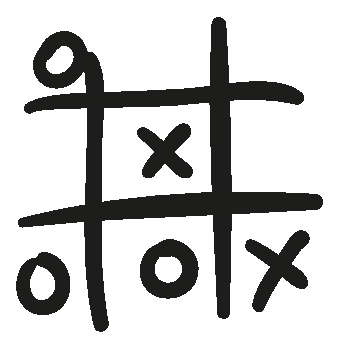
\includegraphics[width=\linewidth]{Images/tic-tac-toe-hand-drawn-game.eps}\\
	\end{columns}
\end{frame}

\begin{frame}{Example: Tic-Tac-Toe}
	\begin{columns}
	\column{0.7\textwidth}
		Play many games against the opponent: Use greedy moves with prohability $1 - \epsilon$ and explorative moves with prohability $\epsilon$.
		Update values after every greedy move:\\
	\vspace{0.5cm}
	\begin{alertblock}{State Value Update Rule}
		$V(S_t) \leftarrow V(S_t) + \alpha[V(S_{t+1}) - V(S_{t})]$\\
	\end{alertblock}
		This is a form of temporal differences learning and a state value method.
	\column{0.3\textwidth}
		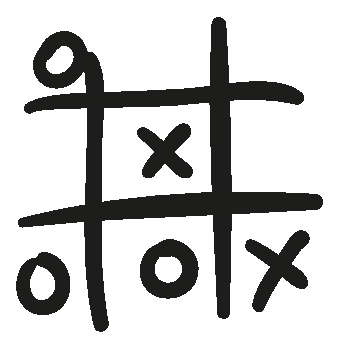
\includegraphics[width=\linewidth]{Images/tic-tac-toe-hand-drawn-game.eps}\\
	\end{columns}
\end{frame}

\begin{frame}{Example: Tic-Tac-Toe}
	\begin{columns}
	\column{0.7\textwidth}
	\centering
	\includegraphics[width=0.85\linewidth]{Images/tictactoe2.png}\\
	\begin{alertblock}{State Value Update Rule}
		$V(S_t) \leftarrow V(S_t) + \alpha[V(S_{t+1}) - V(S_{t})]$\\
	\end{alertblock}
	\column{0.3\textwidth}
		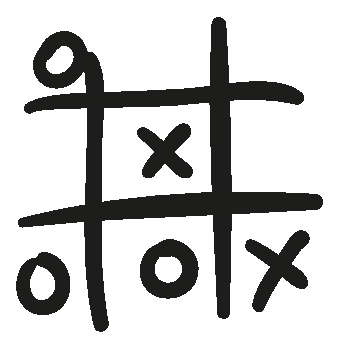
\includegraphics[width=\linewidth]{Images/tic-tac-toe-hand-drawn-game.eps}\\
	\end{columns}
\end{frame}

\begin{frame}{Example: Tic-Tac-Toe}
	\begin{columns}
	\column{0.7\textwidth}
	\begin{alertblock}{State Value Update Rule}
		$V(S_t) \leftarrow V(S_t) + \alpha[V(S_{t+1}) - V(S_{t})]$\\
	\end{alertblock}
	\vspace{0.1cm}
	We reduce the stepsize parameter $\alpha$ over time:\\
	The values converge towards the prohabilities of winning from the current state. \\
	(implementation on github)\\
	\vspace{0.5cm}
	Notice:\\
	\hspace{1cm} Model-free example. \\
	\hspace{1cm} Reward-free example. \\
	\hspace{1cm} No action values.\\
	\hspace{1cm} Suppose opponent makes mistakes.
	\column{0.3\textwidth}
		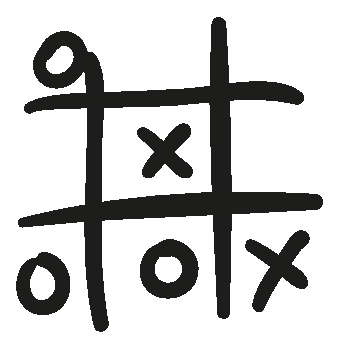
\includegraphics[width=\linewidth]{Images/tic-tac-toe-hand-drawn-game.eps}\\
	\end{columns}

\end{frame}

%----------------------------------------------------------------------------------------
%	 SECTION 2: MULTIARMED BANDIT
%----------------------------------------------------------------------------------------

\section{Multiarmed Bandit Problem}

\begin{frame}{Multiarmed Bandit}
	\begin{columns}
	\column{0.5\textwidth}
	Slot machine with multiple levers, e.g. 10 levers. \\
	\vspace{0.5cm}
	Notice:\\
	\hspace{1cm}Only one possible state.\\
	Objective:\\
	\hspace{1cm}Maximize reward over $k$ timesteps.
	\column{0.5\textwidth}
	\includegraphics[width=\linewidth]{Images/multiarmedbandit.jpg}\\	
	\end{columns}
	%\vspace{0.5cm}
	\begin{block}{Estimate action values:}
		$Q_t(a) = $ (sum of rewards when $a$ taken prior to $t$)/(number of times $a$ taken prior to $t$)
	\end{block}
\end{frame}

\begin{frame}{Reward Distribution}
	\begin{figure}
	\centering
	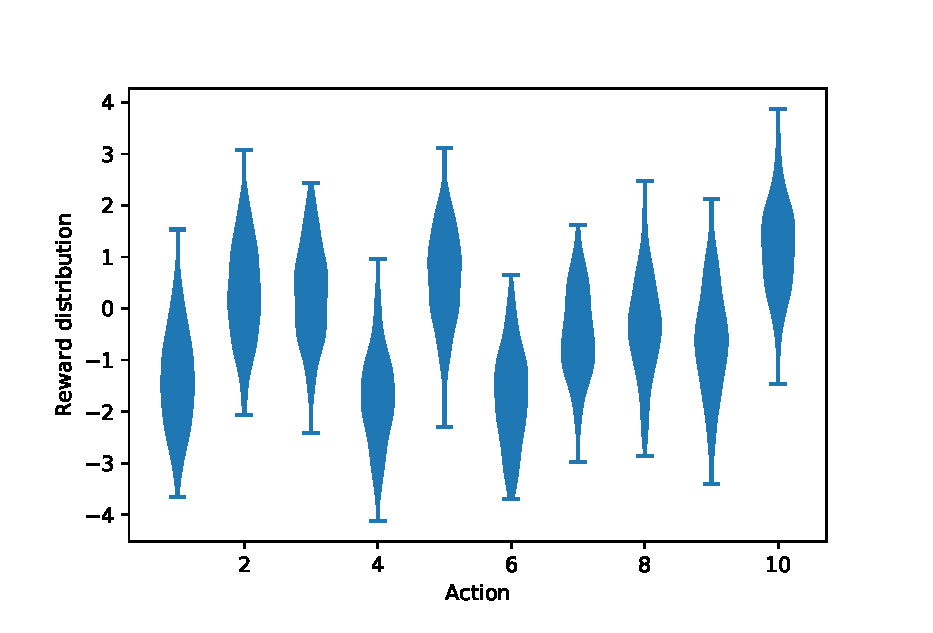
\includegraphics[width=0.8\linewidth]{Images/figure_2_1.eps}\\
	\end{figure}
	Rewards: $R_n \hspace{0.1cm} \propto \hspace{0.1cm} \mathcal{N}(\mu=q_{\asterisk}(n), \sigma=1)$ ... normal distribution\\
	Real Action values: $q_{\asterisk}(n) \hspace{0.1cm} \propto \hspace{0.1cm} \mathcal{N}(\mu=0, \sigma=1)$
\end{frame}

\begin{frame}{Methods for Policy Learning}
	\begin{columns}
	\column{0.7\textwidth}
optimal policy $\pi_{\asterisk}$ ... a policy that maximizes the rewards over time (not necessarily unique!) \\
\vspace{0.3cm}
How to balance exploration and exploitation such that we arraive at an optimal policy?\\
\vspace{0.3cm}
	\column{0.3\textwidth}
	\includegraphics[width=\linewidth]{Images/exploration.jpg} \\[\baselineskip]
	\end{columns} 
Methods (e.g.):
\begin{itemize}
\item $\epsilon$-Greedy Method
\item Optimistic Initial Values
\item UCB Action Selection
\item Gradient Bandit Algorithm
\end{itemize}
\end{frame}

\begin{frame}{$\epsilon$-greedy Method}
	Reminder: \\
	\hspace{0.5cm} Greedy Action ... Action with the highest estimated value.\\
	\vspace{0.5cm}
	\begin{exampleblock}{Algorithm}
	\begin{itemize}
	\item Set up a table with initial estimations for every action value, \\ e.g. $Q(n) = 0$.
	\item Choose $\epsilon \in [0,1]$
	\item For every step:
	\item \hspace{1cm}With probability $\epsilon$ take a random non-greedy action.
	\item \hspace{1cm}Else: Take greedy action and update value.
	\end{itemize}	
	\end{exampleblock}
\end{frame}

\begin{frame}{$\epsilon$-greedy Method}
	Update value according to 
	\begin{block}{Estimate action values:}
		$Q_t(a) = $ (sum of rewards when $a$ taken prior to $t$)/(number of times $a$ taken prior to $t$)
	\end{block}
	
	This can be implemented recursively and efficiently:
	\begin{alertblock}{Action Value Update Rule}
		$ Q_{n+1} = Q_n + \frac{1}{n} \big[ R_n - Q_n \big] $
	\end{alertblock}
	$n$ ... number of times a taken prior to t\\
	 $Q_n$ ... estimation of the true action value $q_{\asterisk}$ after n received rewards\\
	 $R_n$ .. n'th received reward for the action
	
\end{frame}

\begin{frame}{$\epsilon$-greedy Method}
Averaged performance over time step of 2000 indepentend 10 armed bandit problems.
	\begin{figure}
	\centering
	\includegraphics[width=0.6\linewidth]{Images/figure_2_2_a-crop.pdf}
	\end{figure}
\end{frame}

\begin{frame}{$\epsilon$-greedy Method}
Averaged performance over time step of 2000 indepentend 10 armed bandit problems.
	\begin{figure}
	\centering
	\includegraphics[width=0.6\linewidth]{Images/figure_2_2_b-crop.pdf}
	\end{figure}
\end{frame}

\begin{frame}{Optimistic Initial Values}
	Only one difference to $\epsilon$-greedy method:
	\begin{exampleblock}{Algorithm}
	\begin{itemize}
	\item Set up a table with \textbf{unrealistic high}  initial estimations for every action value, \\ e.g. $\mathbf{Q(n) = 5}$.
	\item Choose $\epsilon \in [0,1]$
	\item For every step:
	\item \hspace{1cm}With probability $\epsilon$ take a random non-greedy action.
	\item \hspace{1cm}Else: Take greedy action and update value.
	\end{itemize}	
	\end{exampleblock}
	In the pure version, optimistic value method uses $\epsilon = 0$. 
\end{frame}

\begin{frame}{Optimistic Initial Values}
Averaged performance over time step of 2000 indepentend 10 armed bandit problems.
	\begin{figure}
	\centering
	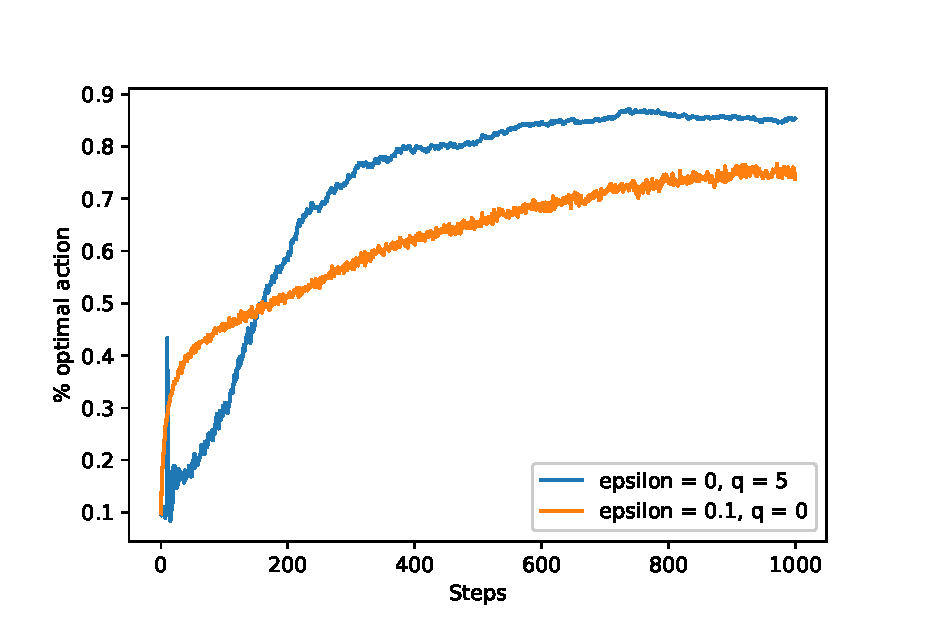
\includegraphics[width=0.9\linewidth]{Images/figure_2_3.eps}\\	
	\end{figure}
\end{frame}

\begin{frame}{Upper Confidence Bound Action Selection}
	Until now, we distiguished between greedy and non-greedy actions. Now we look closer: \\
	\vspace{0.2cm}
	Select between non-greedy actions according to their potential for beeing optimal.  This depends on: \\
	\begin{itemize}
	\item How close is their estimate to being maximal.
	\item Uncertainties in those estimates.
	\end{itemize}

	\begin{alertblock}{Action Selection Rule}
		$A_t = arg \max\limits_{a}  \big[ Q_t (a) + c \sqrt{\frac{ln (t)}{N_t (a)}} \big] $
	\end{alertblock}

	$N_t(a)$ ... number of times a was selected prior to time step $t$ \\
	$c > 0$ ... controls the degree of exploration \\
	If $N_t(a) = 0$,  then $a$ is considered to be an maximizing action.

\end{frame}

\begin{frame}{Upper Confidence Bound Action Selection}
Averaged performance over time step of 2000 indepentend 10 armed bandit problems.
	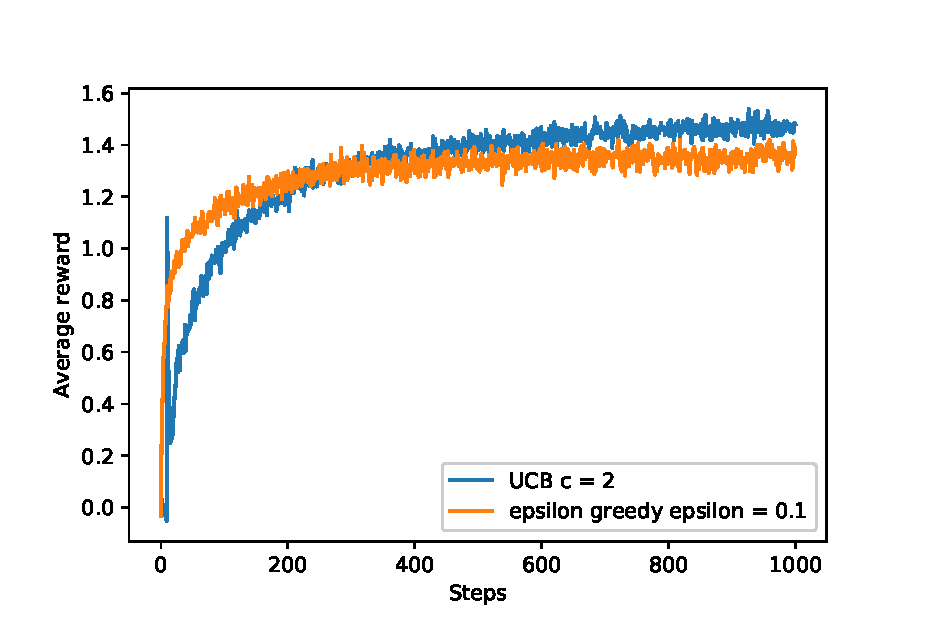
\includegraphics[width=0.9\linewidth]{Images/figure_2_4.eps}\\	
\end{frame}

\begin{frame}{Gradient Bandit Algorithms}
	Value function $q(a)$ is an estimation of the rewards to come. \\
	Different approach: Learn preferences $H_t (a)$ for the actions instead of values. Only their relative difference is relevant! \\
	\begin{alertblock}{Action Selection Rule (Probabilistic!)}
		$Pr\{ A_t = a \} = \frac{ e^{H_t (a)} }{  \sum_{b=1}^{k} e^{H_t (b)} } = \pi_t (a)$
	\end{alertblock}

	\begin{alertblock}{Preferences Update Rule}
		$ H_{t+1} (A_t) = H_t(A_t) + \alpha (R_t - \overline{R_t})(1 - \pi_t (A_t)) $, and \\
		$ H_{t+1} (a) = H_t(a) + \alpha (R_t - \overline{R_t})\pi_t (a) $ for all $a \ne A_t$
	\end{alertblock}	
	
	$\alpha > 0$ ... step size parameter\\
	$\overline{R}_t \in \mathbb{R}$ ... average of all rewards including step $t$ (``baseline'') 
	
\end{frame}

\begin{frame}{Gradient Bandit Algorithms}
Averaged performance over time step of 2000 indepentend 10 armed bandit problems. Here, the true values $q_{\asterisk}(a)$ are $ \propto \hspace{0.2cm} \mathcal{N}(4,1)$. With baseline this makes no difference on the performance.
	\begin{figure}
	\centering
	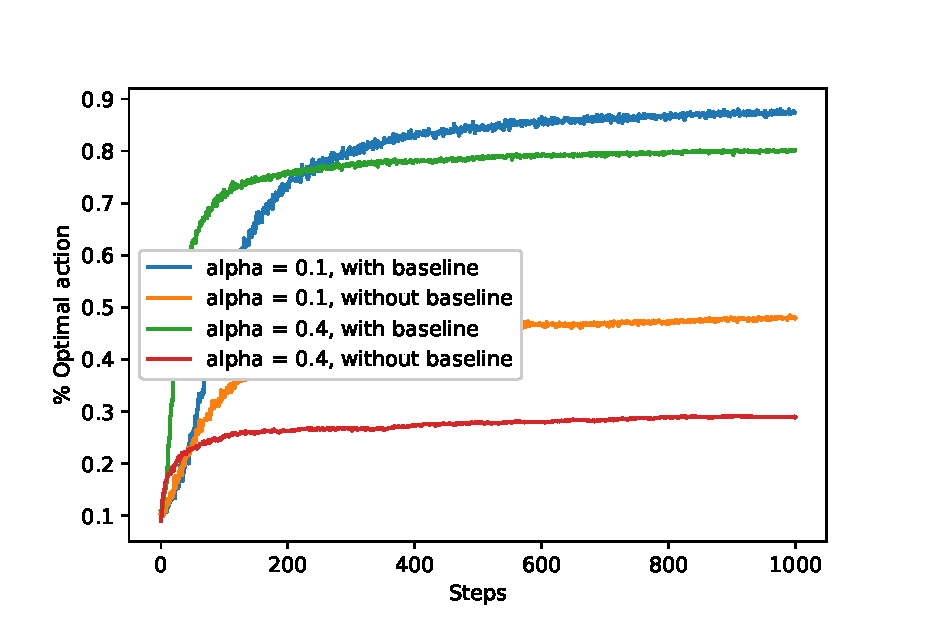
\includegraphics[width=0.75\linewidth]{Images/figure_2_5.eps}\\	
	\end{figure}
\end{frame}

\begin{frame}{Comparison of the Methods}
Parameter Study: Summarize the learning curves by averaging over the first 1000 steps. Parameters: $\epsilon$ ($\epsilon$-greedy), $\alpha$ (gradient bandit), $c$ (UCB), $Q_0$ (optimistic initialization)
	\begin{figure}
	\centering
	\includegraphics[width=0.85\linewidth]{Images/figure_2_6.eps}\\
	\end{figure}
\end{frame}

\begin{frame}{Recap: Policies}
All the algorithms have a policy $\pi$ that tells the algorithm which action in which state to choose (can also be probabilistic).
\begin{itemize}
\item $\epsilon$-Greedy: $\pi(a_{greedy})=1-\epsilon$, $\pi(a_{non-greedy})=\epsilon$
\item Optimistic Initial Values: same as $\epsilon$-Greedy
\item UCB Action Selection: $A_t = arg \max\limits_{a}  \big[ Q_t (a) + c \sqrt{\frac{ln (t)}{N_t (a)}} \big] $
\item Gradient Bandit Algorithm: $\pi_t (a) = \frac{ e^{H_t (a)} }{  \sum_{b=1}^{k} e^{H_t (b)} } $
\end{itemize}
\end{frame}

\begin{frame}{Recap: Update Rules, Values and Preferences}
We want the policy to improve over time, so there is always an update rule for the policy.
\begin{itemize}
\item action value methods: $ Q_{n+1} = Q_n + \frac{1}{n} \big[ R_n - Q_n \big] $
\item action preference methods: $ H_{t+1} (A_t) = H_t(A_t) + \alpha (R_t - \overline{R_t})(1 - \pi_t (A_t)) $, and $ H_{t+1} (a) = H_t(a) + \alpha (R_t - \overline{R_t})\pi_t (a) $ for all $a \ne A_t$
\end{itemize}

In the Tic Tac Toe Example we learned State Values $V(S_t)$, in the Bandit Problem we learned Action Values $Q_t (a)$. In the Gradient Bandit we learned Action Preferences instead of values.

	\begin{alertblock}{General Form for Update Rules}
		$NewEstimate \leftarrow OldEstimate + Stepsize \big[ Target - OldEstimate \big] $
	\end{alertblock}

\end{frame}

%----------------------------------------------------------------------------------------
%	 SECTION 3: FINITE MDPs
%----------------------------------------------------------------------------------------

\section{Finite Markov Decision Processes}

\begin{frame}{Motivation}
Generalization and rigorous framework for the Reinforcement Learning Problem. \\

\begin{figure}
\centering
\includegraphics[width=0.9\linewidth]{Images/AgentEnvironment.png} \\
\end{figure}
Trajectory:\\
$S_0 \rightarrow A_0 \rightarrow \{ R_{1}, S_1 \} \rightarrow A_1 \rightarrow \{ R_{2}, S_2 \} \rightarrow A_2 \rightarrow \{ R_{3}, S_{4} \} ...$

\end{frame}

\begin{frame}{Markov Decision Process}

Def.: State ``space'' $\mathcal{S} $, action space $\mathcal{A}$ and reward space $\mathcal{R}$. We assume all as finite, the theory also works for countable infinite.\\
\vspace{0.3cm}
A Markov decision process is a $4$-tuple $(\mathcal{S}, \mathcal{A}, p, r)$, where \\
\begin{itemize}
\item $p: \begin{cases}\mathcal{S} \times \mathcal{R} \times \mathcal{S} \times \mathcal{A} \rightarrow [0,1] \\ (s',r ,s,a ) \mapsto Pr\{S_t = s', R_t = r| S_{t-1} = s, A_{t-1} = a\}  \end{cases} $ \\ is the dynamics function (conditional probability!). \\
\item $r: \begin{cases} \mathcal{S} \times \mathcal{A} \times \mathcal{S} \rightarrow \mathcal{R} \\ (s, a, s') \mapsto r(s, a, s') \end{cases}$ \\ is the expected reward received after transitioning from state $s$ to state $s'$, due to action $a$.\\
\end{itemize}

\end{frame}

\begin{frame}{Markov Decision Process}

	\begin{columns}
	\column{0.4\textwidth}
	Two important characterstics:
	\begin{itemize}
	\item Well defined prohabilities for all possible transitions.
	\item Each state has the Markov Property: The prohabilities depend only on the current state, not on the past states. The state holds all necessary information for the future.
	\end{itemize}	
	\column{0.6\textwidth}
	\begin{figure}
	\centering
	\includegraphics[width=\linewidth]{Images/Markov_Decision_Process.pdf}\\
	\end{figure}
	\end{columns}

\end{frame}

\begin{frame}{Returns and Discouting}
	The agent seeks to maximize the expected rewards: \\
	\begin{alertblock}{Return}
	$G_t$, a function of the rewards, expected after time step t.\\
	Simples case: $G_t = R_{t+1} + R_{t+2} + \dots + R_T$
	\end{alertblock}
	Simple sum makes only sense for episodic task (task ends after finitely many steps).
	For continuing task: Introduce discounting rate $\gamma \in [0,1]$ and discounted return:\\ 
	\begin{equation*}
	G_t = \sum_{k=0}^{\infty} \gamma^k R_{t+k+1} \hspace{0.5cm} \text{(converges)}
	\end{equation*}
	Returns satisfy recursive relation: $G_t = R_{t+1} + \gamma G_{t+1}$ \\
\end{frame}

\begin{frame}{Continuing and Episodic Tasks}
	Example of continuing task: Pole balancing\\
	Idea for Rewards: $R=-1$ everytime failure occures, else $R=0$
	\begin{columns}
	\column{0.5\textwidth}
	Possible actions: accelerate left and right\\
	State: Angle of the pole to the floor, position on x-axis\\
	\column{0.5\textwidth}	
	\begin{figure}
	\centering
	\includegraphics[width=\linewidth]{Images/pole.png}\\	
	\end{figure}
	\end{columns}
\end{frame}

\begin{frame}{Policies and Value Functions}
	The policy $\pi$ is a mapping from states to probabilities of selecting each possible action:
	\begin{alertblock}{Policy}
	$\pi(a|s) = Pr(A_t = a | S_t = s)$
	\end{alertblock}
	Reminder:\\
	Value function is the expected return when starting in $s$ and following $\pi$ thereafter:  
	 \begin{equation*}
	v_{\pi} (s) = \mathbb{E}\big[ G_t | S_t = s \big] = \mathbb{E}\big[ \sum_{k=0}^{\infty} \gamma^k R_{t+k+1} | S_t = s \big]
	\end{equation*}
	Action value function is the expected return when starting in $s$, taking $a$ and following $\pi$ thereafter:  
	 \begin{equation*}	
	q_{\pi} (s,a) = \mathbb{E}\big[ G_t | S_t = s, A_t = a \big] = \mathbb{E}\big[ \sum_{k=0}^{\infty} \gamma^k R_{t+k+1} | S_t = s, A_t = a  \big] 
	\end{equation*}
\end{frame}

\begin{frame}{Policy and reduction to Markov Chain}

	\begin{columns}
	\column{0.5\textwidth}

MDP's are a generalization of markov chains, they introduce more than one possible action in any state. Together with a fixed policy the MPD reduces to a Markov chain.

	\column{0.5\textwidth}

	\begin{figure}
	\centering
	\includegraphics[width=\linewidth]{Images/markov_chain.png}\\
	\end{figure}

	\end{columns}

\end{frame}

\begin{frame}{Bellman Equation}
	The value function satisfies a recursive relation as well:
	\begin{align}
	v_{\pi}(s) &= \mathbb{E} \big[ G_t | S_t = s \big] \\
	&= \mathbb{E} \big[ R_{t+1} + \gamma G_{t+1} | S_t = s \big]\\
	&= \sum_a \pi (a|s) \sum_{s'} \sum_{r} p(s',r|s,a) \big[ r + \gamma \mathbb{E} [ G_{t+1} | S_{t+1} = s' ] \big] \\
	&= \sum_a \pi(a|s) \sum_{s',r} p(s',r|s,a) \big[ r + \gamma v_{\pi}(s')  \big] \label{bell}
	\end{align} 

	The result is called the

	\begin{exampleblock}{Bellman Equation}
	$v_{\pi}(s) = \sum_a \pi(a|s) \sum_{s',r} p(s',r|s,a) \big[ r + \gamma v_{\pi}(s')  \big] \label{bell} $
	\end{exampleblock}
	
	The value function $v_{\pi}$ is its unique solution and can be found by solving the system of linear equations. For larger systems, there are various methods of learning $v_{\pi}$. 
	\end{frame}

\begin{frame}{Gridworld with Random Policy}
	Example: $5 \times 5$ Grid. \\
	Possible actions: ${u,l,d,r}$ \\
	Rewards: $R=\begin{cases}-1 & \text{for bumping into the walls,} \\ 10 & \text{for jump from A to A',} \\ 5 & \text{for jump from B to B',} \\ 0 & \text{else}  \end{cases}$ \\
	Policy: Choose action from  uniform distribution.
	\begin{figure}
	\centering
	\includegraphics[width=0.9\linewidth]{Images/gridworldrandom.png}\\	
	\end{figure}
\end{frame}

\begin{frame}{Gridworld with Random Policy}
	Compare with code from github: Same results.
	\begin{figure}
	\centering
	\includegraphics[width=0.8\linewidth]{Images/figure_3_2.png}\\	
	\end{figure}
\end{frame}

\begin{frame}{Optimal Policies and Optimal Value Functions}	

\begin{alertblock}{Optimal Policies}
Def.: A policy $\pi$ is better than $\pi'$ if $v_{\pi} (s) \ge v_{\pi'} (s)$ for all $s$. 
An optimal policy $\pi_{\asterisk}$ is better than or equal to all others. There is always at least one such. 
\end{alertblock}
Optimal policies are sharing the same optimal action value function $q_{\asterisk}(s,a) = \max\limits_{\pi} q_{\pi} (s,a)$ for all $a,s$. (unique!)\\
For the state action pair $(s,a)$ this function gives the expected return for taking action $a$ in state $s$ and thereafter following an optimal policy:
\begin{equation*}
q_{\asterisk}(s,a) = \mathbb{E} \big[ R_{t+1} + \gamma v_{\asterisk}(S_{t+1}) | S_t=s, A_t = a \big]
\end{equation*}
\end{frame}

\begin{frame}{Bellman Optimality Equation}	
	Bellman equation for $v_{\asterisk}$ is called Bellman optimality equation:
	\begin{align}
	v_{\asterisk} (s) &= \max\limits_{a} q_{\pi_{\asterisk}} (s,a) \\
	&= \max\limits_{a} \mathbb{E}_{\pi_{\asterisk}} \big[ G_t | S_t =s, A_t = a \big]\\
	&= \max\limits_{a} \mathbb{E}_{\pi_{\asterisk}} \big[ R_{t+1} + \gamma G_{t+1} | S_t =s, A_t = a \big]\\
	&= \max\limits_{a} \mathbb{E} \big[ R_{t+1} + \gamma v_{\asterisk} (S_{t+1}) | S_t =s, A_t = a \big] \label{bellopt1}\\
	&= \max\limits_{a} \sum_{s',r} p(s',r | s,a) \big[ r + \gamma v_{\asterisk} (s') \big] \label{bellopt2}
	\end{align}

Bellman optimality equation for $q_{\asterisk}$:

	\begin{align}
	q_{\asterisk} (s,a) &= \mathbb{E} \big[ R_{t+1} + \gamma \max\limits_{a'} q_{\asterisk} (S_{t+1}, a') | S_t =s, A_t = a \big] \\
	&= \sum_{s',r} p(s',r | s,a) \big[ r + \gamma  \max\limits_{a'} q_{\asterisk} (s', a') \big] 
	\end{align}

\end{frame}

\begin{frame}{Gridworld with Optimal Policy}
	The Bellman Optimality Equation is again just a system of linear equations. Solved Bellman equation for $v_{\asterisk}$ in the Gridworld Example: The value function is unique, the policy isn't.
	\begin{figure}
	\centering
	\includegraphics[width=\linewidth]{Images/gridworldoptimal.png}\\	
	\end{figure}
\end{frame}

\begin{frame}{Gridworld with Optimal Policy}
	Compare with code from github: Same results.
	\begin{figure}
	\centering
	\includegraphics[width=0.8\linewidth]{Images/figure_3_5.png}\\	
	\end{figure}	
\end{frame}

\begin{frame}{Recap: Finite MDP}

\textbf{Finite MDP}: Finite set of states, actions and rewards together with well defined transition prohabilities, depending on the current state and the taken action. The current state holds all information about the past (Markov Property). \\
\textbf{Policy}: Tells the agent which action to take in which state. \\
\textbf{Return}: Estimation of the future rewards. \\
\textbf{(Action) Value function}: Assign estimated Returns to states (action state pairs). \\
\textbf{Bellman Equation}: Recursive relation of the value function, can be solved as system of linear equations. \\
\vspace{0.3cm}
What was not in this chapter? \\
Strategies to arrive at an optimal policy!\\
Before: Update rules for Tic Tac Toe and Multiarmed Bandit were strategies to solve the Bellman Equation and arrive at an optimal policy at the same time.

\end{frame}

%----------------------------------------------------------------------------------------
%	 SECTION 4: PROJECTS
%----------------------------------------------------------------------------------------

\section{Projects}

\begin{frame}{Labyrinth Escape}
	\begin{columns}
	\column{0.7\textwidth}
	Agent starts at the red cross and needs to escape the labyrinth.\\
	\vspace{0.5cm}
	Possible actions: $\{ U, R, D, L \}$ \\
	\vspace{0.5cm}
	Rewards: \\
	\hspace{1cm} Bump into wall: $R = -1$ \\
	\hspace{1cm} Escape: $R = 100$ \\
	\hspace{1cm} Other actions: $R = 0$ \\
	\column{0.3\textwidth}
	\includegraphics[width=\linewidth]{Images/sketch.png}\\	
	\end{columns}	
\end{frame}

\begin{frame}{Labyrinth Escape}
	$\epsilon$-greedy method, with over episodes linearily decreasing $\epsilon \in [0,1]$.
	\begin{exampleblock}{Q-Learning Algorithm}
	Define q-table containing a field for every action-state value.\\
	\vspace{0.3cm}
	Update action-state values after every greedy action:
	\vspace{0.3cm}
	$Q(s_t,a_t) \leftarrow (1 - \alpha) Q(s_t,a_t) + \alpha[R(s_t,a_t) + \gamma \max\limits_a Q(s_{t+1},a)]$	
	\end{exampleblock}
	$\alpha$ ... Learning Rate, $\gamma$ ... Discounting Factor \\
	Notice: The value update rule is actually the Bellman Equation. 
\end{frame}

\begin{frame}{Labyrinth: Learning Curve}
	After 30 episodes the agent finds an optimal policy.
	\begin{figure}
	\centering
	\includegraphics[width=0.7\linewidth]{Images/learning_curve.eps}\\	
	\end{figure}
\end{frame}

\begin{frame}{Labyrinth: Action Values}
	Action values, learned by the q learning algorithm.
	\begin{figure}
	\centering
	\includegraphics[width=0.7\linewidth]{Images/direction_values.eps}\\	
	\end{figure}
\end{frame}

\begin{frame}{Labyrinth: Greedy Directions}
	Greedy actions for every state.
	\begin{figure}
	\centering
	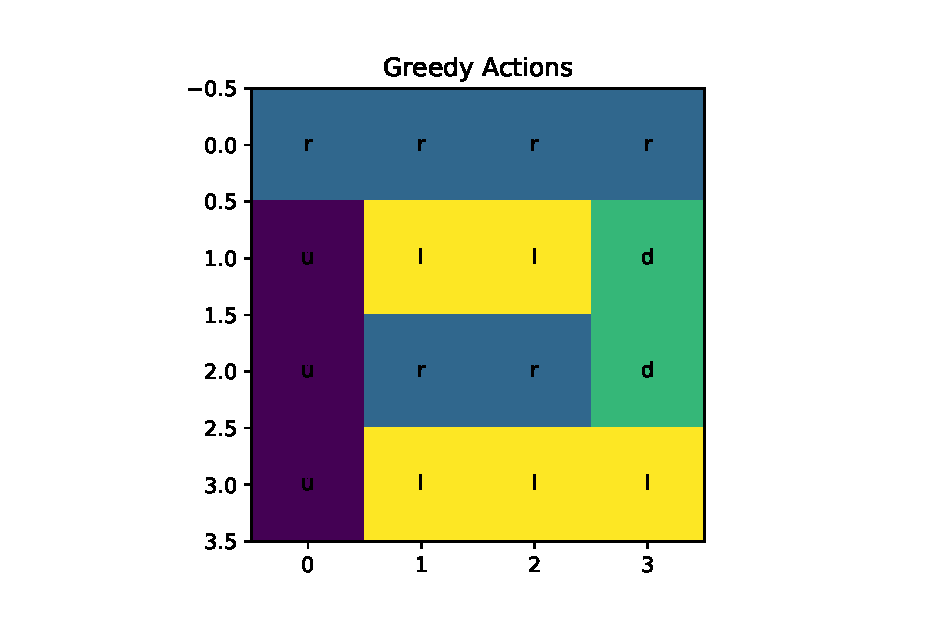
\includegraphics[width=0.7\linewidth]{Images/greedy_directions.eps}\\	
	\end{figure}
\end{frame}

%----------------------------------------------------------------------------------------
%	 SECTION 4: PROJECTS, TRAVELLING SALESMAN
%----------------------------------------------------------------------------------------

\begin{frame}{Travelling Salesman Problem (ongoing work)}
	A Salesman wants to visit certain cities (e.g. all capitital cities in austria) while driving as less kilometers as possible. \\
	%\vspace{0.5cm}
	\begin{columns}
	\column{0.6\textwidth}
	Set Startpoint and wanted endpoint.\\
	Define Q-table for action-state values.\\
	Consider Markov Property! \\State = \{ current city , cities already visited \}\\
	\column{0.4\textwidth}
	\begin{figure}
	\centering
	\includegraphics[width=\linewidth]{Images/osterreich.jpg}	
	\end{figure}
	\end{columns}
	Set Rewards:\\
	\hspace{1cm}$R(\text{A to B})$ = $- \text{(distance in kilometers)}$\\
	\hspace{1cm}$R(\text{arriving at endponit when all cities visited}) = 10000$\\
	Update Rule as above.	
\end{frame}

\begin{frame}{Travelling Salesman Problem (ongoing work)}
to be continued ... (on github and in the paper!) \\
\vspace{1 cm}
\begin{figure}
\centering
\includegraphics[width=0.4\linewidth]{Images/WORK-IN-PROGRESS.jpg}	
\end{figure}
\end{frame}

%----------------------------------------------------------------------------------------
%	 CLOSING/SUPPLEMENTARY SLIDES
%----------------------------------------------------------------------------------------

\begin{frame}{References}
	\begin{columns}
	\column{0.6\textwidth}
	Sutton S. Barto \& Andrew G. Barto, Reinforcement Learning: An Introduction
	\column{0.4\textwidth}
	\includegraphics[width=\linewidth]{Images/suttonbarto.png}\\	
	\end{columns}
	\vspace{0.2cm}
	Implementation of Sutton \& Barto's examples on github: \\
	github.com/ShangtongZhang/reinforcement-learning-an-introduction\\
	\vspace{0.2cm}
	Presentation and Implementation of Labyrinth \& Travelling Salesman on github:
	github.com/fewagner/ReinforcementLearning \\
	\vspace{0.2cm} 
	Presentation template from http://www.LaTeXTemplates.com (Pasquale Africa), some icons made by Freepik from www.flaticon.com, some pictures taken from Wikipedia
\end{frame}

\begin{frame}[focus]
	Questions?
\end{frame}

%----------------------------------------------------------------------------------------
\appendix


%\begin{frame}[plain]{Plain Slide}
%	This is a slide with the plain style and it is numbered.
%\end{frame}
%
%%------------------------------------------------
%
%\begin{frame}[t]
%	This slide has an empty title and is aligned to top.
%\end{frame}

%------------------------------------------------
 
%\begin{frame}[noframenumbering]{No Slide Numbering}
%	This slide is not numbered and is citing reference \cite{knuth74}.
%\end{frame}

%------------------------------------------------

%\begin{frame}{Typesetting and Math}
%	The packages \texttt{inputenc} and \texttt{FiraSans}\footnote{\url{https://fonts.google.com/specimen/Fira+Sans}}\textsuperscript{,}\footnote{\url{http://mozilla.github.io/Fira/}} are used to properly set the main fonts.
%	\vfill
%	This theme provides styling commands to typeset \emph{emphasized}, \alert{alerted}, \textbf{bold}, \textcolor{example}{example text}, \dots
%	\vfill
%	\texttt{FiraSans} also provides support for mathematical symbols:
%	\begin{equation*}
%		e^{i\pi} + 1 = 0.
%	\end{equation*}
%\end{frame}

%------------------------------------------------

%\begin{frame}{Blocks}
%	These blocks are part of 1 slide, to be displayed consecutively.
%	\begin{block}{Block}
%		Text.
%	\end{block}
%	\pause % Automatically creates a new "page" split between the above and above + below
%	\begin{alertblock}{Alert block}
%		Alert \alert{text}.
%	\end{alertblock}
%	\pause % Automatically creates a new "page" split between the above and above + below
%	\begin{exampleblock}{Example block}
%		Example \textcolor{example}{text}.
%	\end{exampleblock}
%\end{frame}

%------------------------------------------------

%\begin{frame}{Columns}
%	\begin{columns}
%		\column{0.5\textwidth}
%			This text appears in the left column and wraps neatly with a margin between columns.
%		
%		\column{0.5\textwidth}
%			\includegraphics[width=\linewidth]{Images/placeholder.jpg}
%	\end{columns}
%\end{frame}

%------------------------------------------------

%\begin{frame}{Lists}
%	\begin{columns}[T, onlytextwidth] % T for top align, onlytextwidth to suppress the margin between columns
%		\column{0.33\textwidth}
%			Items:
%			\begin{itemize}
%				\item Item 1
%				\begin{itemize}
%					\item Subitem 1.1
%					\item Subitem 1.2
%				\end{itemize}
%				\item Item 2
%				\item Item 3
%			\end{itemize}
%		
%		\column{0.33\textwidth}
%			Enumerations:
%			\begin{enumerate}
%				\item First
%				\item Second
%				\begin{enumerate}
%					\item Sub-first
%					\item Sub-second
%				\end{enumerate}
%				\item Third
%			\end{enumerate}
%		
%		\column{0.33\textwidth}
%			Descriptions:
%			\begin{description}
%				\item[First] Yes.
%				\item[Second] No.
%			\end{description}
%	\end{columns}
%\end{frame}

%------------------------------------------------

%\begin{frame}{Table}
%	\begin{table}
%		\centering % Centre the table on the slide
%		\begin{tabular}{l c}
%			\toprule
%			Discipline & Avg. Salary \\
%			\toprule
%			\textbf{Engineering} & \textbf{\$66,521} \\
%			Computer Sciences & \$60,005\\
%			Mathematics and Sciences & \$61,867\\
%			\midrule
%			\textbf{Average for All Disciplines} & \textbf{\$58,114}\\
%			\bottomrule
%		\end{tabular}
%	\caption{Table caption}
%	\end{table}
%\end{frame}

%-------------------------------------------------



%------------------------------------------------

%\begin{frame}{Backup Slide}
%	This is a backup slide, useful to include additional materials to answer questions from the audience.
%	\vfill
%	The package \texttt{appendixnumberbeamer} is used to refrain from numbering appendix slides.
%\end{frame}

%----------------------------------------------------------------------------------------

%\begin{frame}{Definition: Filtration}
%
%
%In [[measure theory]], in particular in [[martingale theory]] and the theory of [[stochastic process]]es, a filtration is an increasing [[sequence (mathematics)|sequence]] of [[sigma algebra|<math>\sigma</math>-algebras]] on a [[measurable space]]. That is, given a measurable space <math>(\Omega, \mathcal{F})</math>, a filtration is a sequence of <math>\sigma</math>-algebras <math>\{ \mathcal{F}_{t} \}_{t \geq 0}</math> with <math>\mathcal{F}_{t} \subseteq \mathcal{F}</math> where each <math>t</math> is a non-negative real number and
%
%:<math>t_{1} \leq t_{2} \implies \mathcal{F}_{t_{1}} \subseteq \mathcal{F}_{t_{2}}.</math>
%
%The exact range of the "times" ''<math>t</math>'' will usually depend on context: the set of values for <math>t</math> might be [[discrete set|discrete]] or continuous, [[bounded set|bounded]] or unbounded. For example,
%
%:<math>t \in \{ 0, 1, \dots, N \}, \mathbb{N}_{0}, [0, T] \mbox{ or } [0, + \infty).</math>
%
%\end{frame}
%
%%----------------------------------------------------------------------------------------
%
%\begin{frame}{Definition: Markov Property}
%
%Let <math>(\Omega,\mathcal{F},\mathbb{P})</math> be a [[probability space]] with a [[Filtration (probability theory)|filtration]] <math>(\mathcal{F}_s,\ s \in I)</math>, for some ([[totally ordered]]) index set <math>I</math>; and let <math>(S,\mathcal{S})</math> be a [[measurable space]]. A <math>(S,\mathcal{S})</math>-valued stochastic process <math>X=\{X_t:\Omega \to S\}_{t\in I}</math> [[Adapted process|adapted to the filtration]] is said to possess the ''Markov property'' if, for each <math>A \in \mathcal{S}</math>  and each <math>s,t\in I</math> with <math>s<t</math>,
%
%:<math>\mathbb{P}(X_t \in A \mid \mathcal{F}_s) = \mathbb{P}(X_t \in A\mid X_s).</math><ref>Durrett, Rick. ''Probability: Theory and Examples''. Fourth Edition. Cambridge: Cambridge University Press, 2010.</ref>
%
%In the case where <math>S</math> is a discrete set with the [[Sigma-algebra#Simple set-based examples|discrete sigma algebra]] and <math>I = \mathbb{N}</math>, this can be reformulated as follows:
%
%:<math>\mathbb{P}(X_n=x_n\mid X_{n-1}=x_{n-1}, \dots, X_0=x_0)=\mathbb{P}(X_n=x_n\mid X_{n-1}=x_{n-1}). </math>
%
%\end{frame}

\end{document}
